\section{Durchführung}
\label{sec:Durchführung}

In Abbildung \ref{fig:aufbau} findet sich eine schematische Darstellung der verwendeten 
Messapperatur. Zur Messung der Strahlintensität wird ein Geiger-Müller-Zählrohr
verwendet. Mit Hilfe eines elektronischen Zählwerks kann die Messdauer variiert
werden. Ebenfalls an diesem Gerät kann die gemessene Zählrate abgelesen werden. 
Der Aufbau zur Vermessung einer $^{137}Cs$-Probe, welche $\gamma$-Strahlen 
aussendet, wird aus aus Sicherheitsgründen durch eine Bleiwand abgeschirmt. Der 
Aufbau zur Messung an dem $\beta$-Strahler $^{99}Tc$ wird durch Aluminium 
abgeschirmt. Bevor der eigentliche Versuch beginnt, wird eine Nullmessung zur 
Bestimmung des sogenannten Nulleffektes durchgeführt. Hierzu wird ohne 
eine Strahlungsquelle $\SI{900}{\second}$ lang die Zählrate gemessen.\\

\begin{figure}
  \centering
  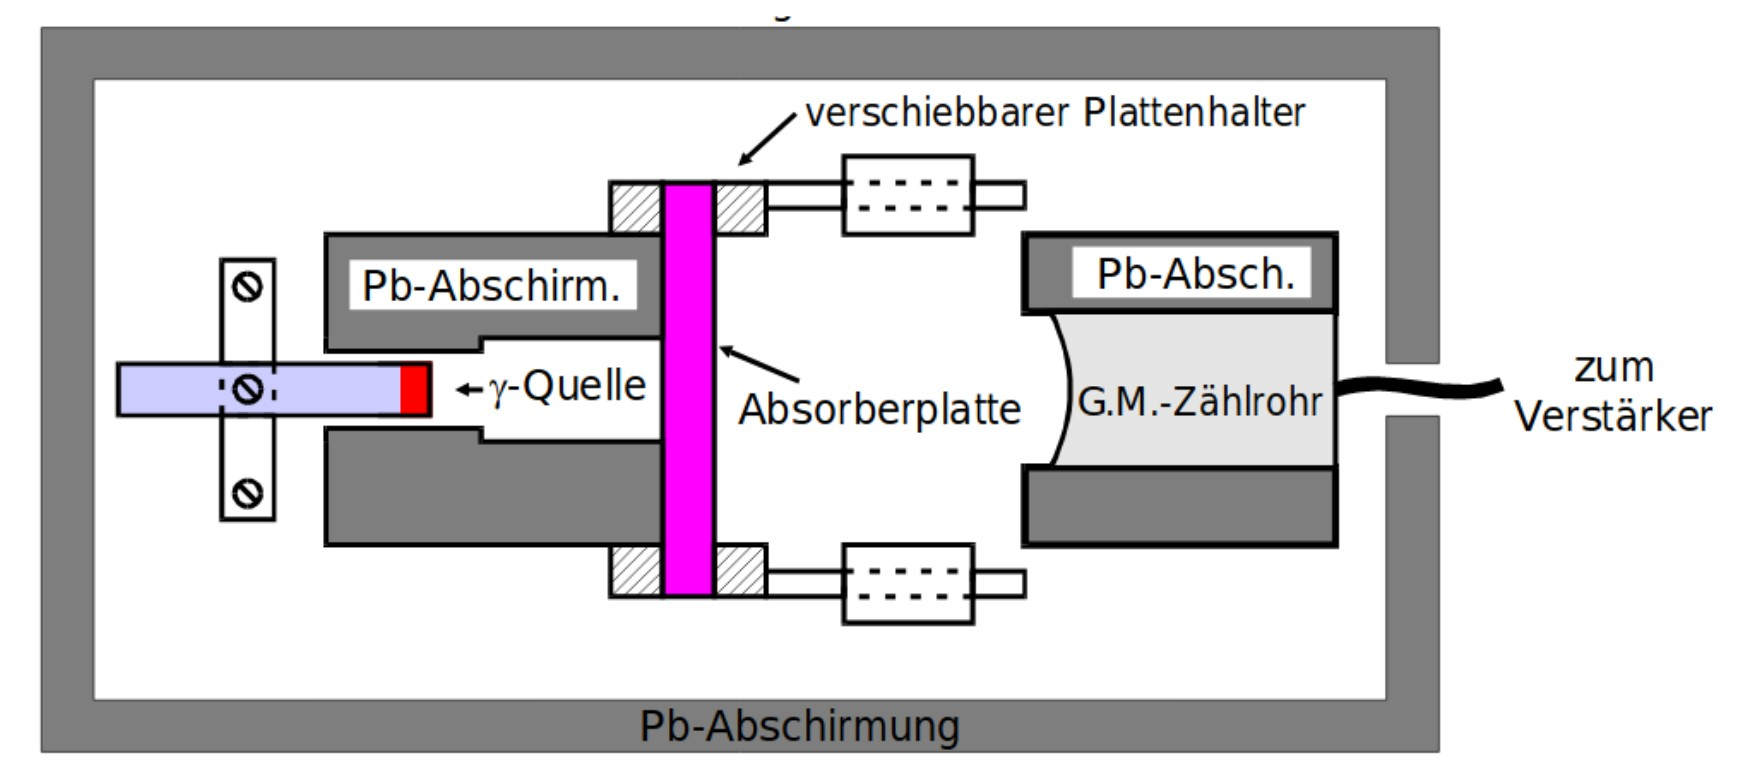
\includegraphics[scale=0.3]{content/Aufbau.jpg}
  \caption{Schmatischer Aufbau der Apperatur zur Vermessung von $\gamma$-Strahlung [1].}
  \label{fig:aufbau}
\end{figure}

Für die Messung an dem $\gamma$-Strahler werden die Materialien Eisen und Blei
als Absorber zwischen Strahlungsquelle und Detektor eingesetzt. Es wird je eine
Messung der Zählrate, die Schichtdicke um circa $\SI{0.5}{\centi\meter}$ erhöht,
und dann wieder eine Messung der Zählrate durchgeführt. Dadurch liegt nach $\num{10}$
Messungen die Schichtdicke bei $\SI{5}{\centi\meter}$. Die Messzeiten
variieren in nahezu gleichmäßigen Abständen von $\SI{40}{\second}$ bis $\SI{500}{\second}$.\\
Für den Versuchsteil mit der Messung an dem $\beta$-Strahler, werden 11 verschiedene 
Aluminiumplatten verschiedener Dicken zur Messung verwendet. Die Messzeiten 
betragen hier zwischen $\SI{100}{\second}$ bis $\SI{500}{\second}$.